\documentclass[a4paper]{article}

%% Language and font encodings
\usepackage[english]{babel}
\usepackage[utf8x]{inputenc}
\usepackage[T1]{fontenc}

%% Sets page size and margins
\usepackage[a4paper,top=3cm,bottom=2cm,left=3cm,right=3cm,marginparwidth=1.75cm]{geometry}

%% Useful packages
\usepackage{amsmath}
\usepackage{graphicx}
\usepackage[colorinlistoftodos]{todonotes}
\usepackage[colorlinks=true, allcolors=blue]{hyperref}
\usepackage{listings}
\usepackage{xcolor}
\lstset { %
    language=C++,
    backgroundcolor=\color{black!5}, % set backgroundcolor
    basicstyle=\footnotesize,% basic font setting
}

\title{Udacity Flying Car Nanodegree 3rd Project\\ 
       Implement Controllers in C++}
\author{Xinjie Qiu \\
        qiuxinjie@gmail.com}
\date{\today}

\begin{document}
\maketitle

\section{Introduction}

The purpose of this project is to write low level controllers for the flight vehicle in C++. This includes implementing controller and tuning control gains. 

\section{Drone Controllers}

To control the drone in three dimension, the following controller architecture is adopted, which consists of \textbf{att}itude controller, \textbf{alt}itude controller, lateral controller. The attitude controller breaks down into smaller controllers responsible for body rate, roll-pitch, and yaw. There are total of 5 controllers to implement in this project. 

\begin{figure}[ht]
\centering
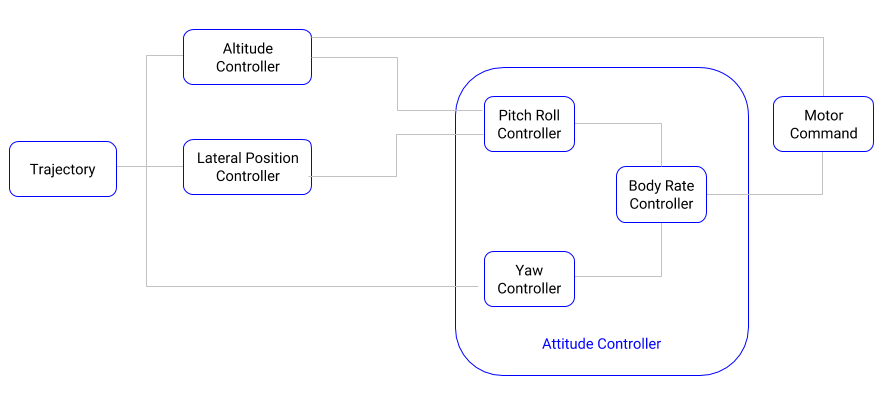
\includegraphics[width=0.9\textwidth]{./fig/ControlArchitecture.png}
\caption{\label{fig:controller} overall control architecture.}
\end{figure}

In the following subsections, each controller will be implemented in C++.

\subsection{body rate control}

Body rate controller is implemented as a P (proportional) controller. It collects commanded roll, pitch, and yaw rates ($p, q, r$), then translates into the desired commanded moments along the axis. 

The control equations have the following form:
$$ \dot{\omega}_{p} = k_{p}^{P} (p_c - p) $$
$$ \dot{\omega}_{q} = k_{p}^{Q} (q_c - q) $$
$$ \dot{\omega}_{r} = k_{p}^{R} (r_c - r) $$
Quantity with subscript c means "commanded" (or "desired") one, without subscript means an "actual" (or more precisely speaking, "estimated") one.

The commanded moments (M, or torque $\tau$ in physics, in unit [$N \cdot m$]) is the product of moment of inertia ($I$, [$kg \cdot m^2$]) and angular acceleration ($\dot{\omega}$, [$radians/s^2$]).
$$ M = I \dot{\omega} $$
The implemented body rate controller is:

\begin{lstlisting}
    V3F momentCmd;
    V3F rate_error = pqrCmd - pqr;
    V3F omega_dot_des = rate_error * kpPQR;
    momentCmd = omega_dot_des * V3F(Ixx, Iyy, Izz);
\end{lstlisting}

\subsection{roll pitch control}
The roll-pitch controller is a P only controller responsible for commanding the roll and pitch rates in the body frame. It uses the lateral acceleration and thrust commands, in addition to the vehicle attitude to output a body rate command. 

This is the trickiest controller to implement due to that it involves rotation matrix from inertial frame to body frame.

The controller first calculates the acceleration in the thrust direction in the body frame $c_d$ by dividing the collective thrust by drone's mass. Then the target angles are calculated from local accelerations. Note both target angles need to be constraint to maximum title angle.
\begin{gather*}
R_{13} = b^x_a = - \ddot{x} / c_d \\
R_{23} = b^y_a = - \ddot{y} / c_d
\end{gather*}
The reason there's a minus sign is due to that the vertical component of thrust is negative in the NED coordinate system.

The desired body rates are then set the rate of change of the given matrix elements using a P controller. 

$$\dot{b}^x_c  = k_p(b^x_c - b^x_a)$$
$$\dot{b}^y_c  = k_p(b^y_c - b^y_a)$$

where $b^x_a = R_{13}$ and $b^y_a = R_{23}$. The given values can be converted into the angular velocities into the body frame by the next matrix multiplication. 

$$
\begin{pmatrix} p_c \\ q_c \\ \end{pmatrix}  = \frac{1}{R_{33}}\begin{pmatrix} R_{21} & -R_{11} \\ R_{22} & -R_{12} \end{pmatrix} \times \begin{pmatrix} \dot{b}^x_c \\ \dot{b}^y_c  \end{pmatrix} 
$$

\begin{lstlisting}
    V3F pqrCmd;
    Mat3x3F R = attitude.RotationMatrix_IwrtB();
    
    float c_d = collThrustCmd/mass;
    float target_R13 = CONSTRAIN(-accelCmd.x/c_d, -maxTiltAngle, maxTiltAngle);
    float target_R23 = CONSTRAIN(-accelCmd.y/c_d, -maxTiltAngle, maxTiltAngle);
    float x_dot_cmd = kpBank*(R(0,2)-target_R13);
    float y_dot_cmd = kpBank*(R(1,2)-target_R23);
    
    pqrCmd.x = (-R(1,0)*x_dot_cmd + R(0,0)*y_dot_cmd)/R(2,2);
    pqrCmd.y = (-R(1,1)*x_dot_cmd + R(0,1)*y_dot_cmd)/R(2,2);
    pqrCmd.z = 0.0;
\end{lstlisting}

\subsection{altitude controller}

In this altitude controller implementation, velocity uses a feed forward P controller,
$$\dot{z} = \dot{z}_c  + k_{p}^{posZ}(z_{c} - z) $$
This vertical component of velocity is constraint between maximum ascent rate and maximum descent rate.

Acceleration uses a feed forward PI controller, which also contains an integrator part to handle the non-ideal center of gravity presented in scenario 4,
$$\ddot{z} = \ddot{z}_c + k_{p}^{velZ}(\dot{z}_{c} - \dot{z}) + k_i^{posZ}\int_0^t(z_{c} - z)dt'$$ 

In the altitude controller, the thrust is controlled through the vertical acceleration. From Newton's second law of motion, the acceleration in z direction is,
$$ m \ddot{z} = - F_{thrust} b^z + m g$$
$g$ is in positive direction, thrust is in negative direction in the NED system. $b^z = R_{33}$ are the the last row last column element in the rotation matrix to translate back from inertial frame to body frame in the case of non-zero roll/pitch angles.
$$ F_{thrust} = m (g - \ddot{z})/b^z$$ 

The C++ implementation code:
\begin{lstlisting}
    float velocityZ = kpPosZ * (posZCmd - posZ) + velZCmd;
    // Limit the ascent/descent rate
    velocityZ = CONSTRAIN(velocityZ, - maxAscentRate, maxDescentRate);
    
    integratedAltitudeError += (posZCmd - posZ) * dt;
    
    float accelerationZ =  accelZCmd
                    + kpVelZ * (velocityZ - velZ)
                    + KiPosZ * integratedAltitudeError;
    
    thrust = mass * (CONST_GRAVITY - accelerationZ) / R(2,2);

\end{lstlisting}

\subsection{lateral position control}
The lateral position control uses two cascaded feed forward P controller to generate a commanded local acceleration from the local NE position, velocity and acceleration.
$$\dot{x} = \dot{x}_c  + k_{p}^{PosXY}(x_{c} - x), \:
  \dot{y} = \dot{y}_c  + k_{p}^{PosXY}(y_{c} - y)$$
$$\ddot{x} = \ddot{x}_c  + k_{p}^{VelXY}(\dot{x_{c}} - \dot{x}), \:
  \ddot{y} = \ddot{y}_c  + k_{p}^{VelXY}(\dot{x_{c}} - \dot{y})$$

\textit{I tried to constraint maximum XY velocity and maximum XY acceleration. But in the later gain tuning part, these constraints prevent the green drone in the $4^{th}$ scenario to reach its target location. For now, I just lift these constraints.}

\begin{lstlisting}
    V3F velocity_xy = velCmd + kpPosXY*(posCmd-pos);
    // Limit speed
    // if (velocity_xy.mag() > maxSpeedXY)
    //        velocity_xy = velocity_xy.norm() * maxSpeedXY;
    
    accelCmd = accelCmd + kpVelXY*(velocity_xy - vel);
    // limit accelaration
    // if (accelCmd.mag() > maxAccelXY)
    //     accelCmd = accelCmd.norm() * maxAccelXY;
\end{lstlisting}

\subsection{yaw control}
The yaw controller is a linear proportional heading controller to yaw rate commands.
The control over yaw is decoupled from the all other directions.
$$ r_c = k_p^{yaw} (\psi_c - \psi) $$

\begin{lstlisting}
    yawCmd = fmodf(yawCmd,M_PI*2.0);
    float yaw_error = AngleNormF(yawCmd - yaw);
    yawRateCmd = kpYaw*yaw_error;
\end{lstlisting}

\subsection{calculate the motor commands given commanded thrust and moments}

Using the desired or estimated position, velocity, attitude, and body rates information sent from the simulator, commands are passed from the above 5 controllers as three directional body moments and thrust. These desired 3-axis moment and collective thrust command are then converted to individual motor thrust commands.

The numbering order of propellers in the C++ project is displayed in figure~\ref{fig:drone1}. 1 is front left, 2 is front right, 3 is rear left, 4 is rear right. Notice this numbering order is different from the lecture exercise and the Python project. Specifically, 3 and 4 are switched. 

\begin{figure}[ht]
\centering
\includegraphics[width=0.5\textwidth]{./fig/drone1.png}
\caption{\label{fig:drone1} Propeller location.}
\end{figure}

Distance from vehicle origin to motors is $L$, the distance from motor to x or y axis is $ l = L/\sqrt[]{2}$. The thrust from each propeller is labeled as $F_1$, $F_2$, $F_3$, $F_4$, the collective thrust is
$$ F_{total} = F_1 + F_2 + F_3 + F_4 $$
For roll motion, the moments generated by the $1^{st}$ and $3^{rd}$ propellers are counteracted by the moment generated by the $2^{nd}$ and the $4^{th}$ propellers. 
$$ \tau_x = (F_1 - F_2 + F_3 - F_4)l $$
In the same fashion, the pitch is generated by the mismatch of the moments created by $1^{st}$ and $2^{nd}$ propellers and the moment generated by the $3^{rd}$ and $4^{th}$ propellers.
$$ \tau_y = (F_1 + F_2 - F_3 - F_4)l $$
Contrary to the roll and pitch, the yaw motion is executed by the mismatch of the moments generated by the propellers along the z axis by the reactive force. The moment generated by the propeller is directed opposite of its rotation and is proportional to the square of the angular velocities. The propellers 1 and 4 rotate in clockwise thus producing the moment in the counterclockwise direction with negative moments. Propellers 2 and 3 rotate in counterclockwise thus the resulting moments are in opposite and have the positive moments.
\begin{align*}
\tau_z &= k_m (-\omega^2_1 + \omega^2_2 + \omega^2_3 - \omega^2_4) \\
       &= -\frac{k_m}{k_f} (F_1 - F_2 - F_3 + F_4) \\
       &= -k_{appa}  (F_1 - F_2 - F_3 + F_4)
\end{align*}

Rearrange these 4 equations, we have
\begin{align*}
F_1 + F_2 + F_3 + F_4 &= F_{total}  \\
F_1 - F_2 + F_3 - F_4 &= \tau_x / l \\
F_1 + F_2 - F_3 - F_4 &= \tau_y / l \\
F_1 - F_2 - F_3 + F_4 &= -\tau_z / k_{appa}
\end{align*}

Quantities on the left side are unknown, on the right side are konwn. Solve these 4 equations for thrust from each propeller,
\begin{align*}
F_1 = (F_{total} + \tau_x / l + \tau_y / l  -\tau_z / k_{appa})/4  \\
F_2 = (F_{total} - \tau_x / l + \tau_y / l  +\tau_z / k_{appa})/4 \\
F_3 = (F_{total} + \tau_x / l - \tau_y / l  +\tau_z / k_{appa})/4 \\
F_4 = (F_{total} - \tau_x / l - \tau_y / l  -\tau_z / k_{appa})/4
\end{align*}

Motor command implementation in C++:
\begin{lstlisting}
    float lenth = L / sqrtf(2);
    float F_total = collThrustCmd;
    float F_x     = momentCmd.x / lenth;
    float F_y     = momentCmd.y / lenth;
    float F_z     = - momentCmd.z / kappa;
    cmd.desiredThrustsN[0] = (F_total + F_x + F_y + F_z) / 4.f; // front left, [N]
    cmd.desiredThrustsN[1] = (F_total - F_x + F_y - F_z) / 4.f; // front right
    cmd.desiredThrustsN[2] = (F_total + F_x - F_y - F_z) / 4.f; // rear left
    cmd.desiredThrustsN[3] = (F_total - F_x - F_y + F_z) / 4.f; // rear right
\end{lstlisting}

\section{Flight Control Gain Tuning}

The C++ controller is able to fly the provided test trajectory and visually passes inspection of the scenarios leading up to the test trajectory.

\subsection{Intro (scenario 1)}

\subsection{Body rate and roll/pitch control (scenario 2)}

\subsection{Position/velocity and yaw angle control (scenario 3)}

\subsection{Non-idealities and robustness (scenario 4)}

\subsection{Tracking trajectories (scenario 5)}


\end{document}